\documentclass{article}

\title{Laboratorio - esercizio con ladder}
\date{}

\usepackage{tabularx} %per le tabelle
\usepackage{booktabs} %per le linee
\usepackage[italian]{babel}  % Lingua
\usepackage{graphicx} %per le immagini
\usepackage{pdfpages} %include pdf
\usepackage{amsmath} %uso simboli matematici
\usepackage{caption}
\usepackage{float}


\title{Laboratorio - Esercizio con Testo Strutturato}
\author{Benedetta Vitale ed Emilio Meroni}
\date{18 maggio 2024}


\begin{document}

\maketitle

\tableofcontents

\begin{figure}[b]
    \centering
    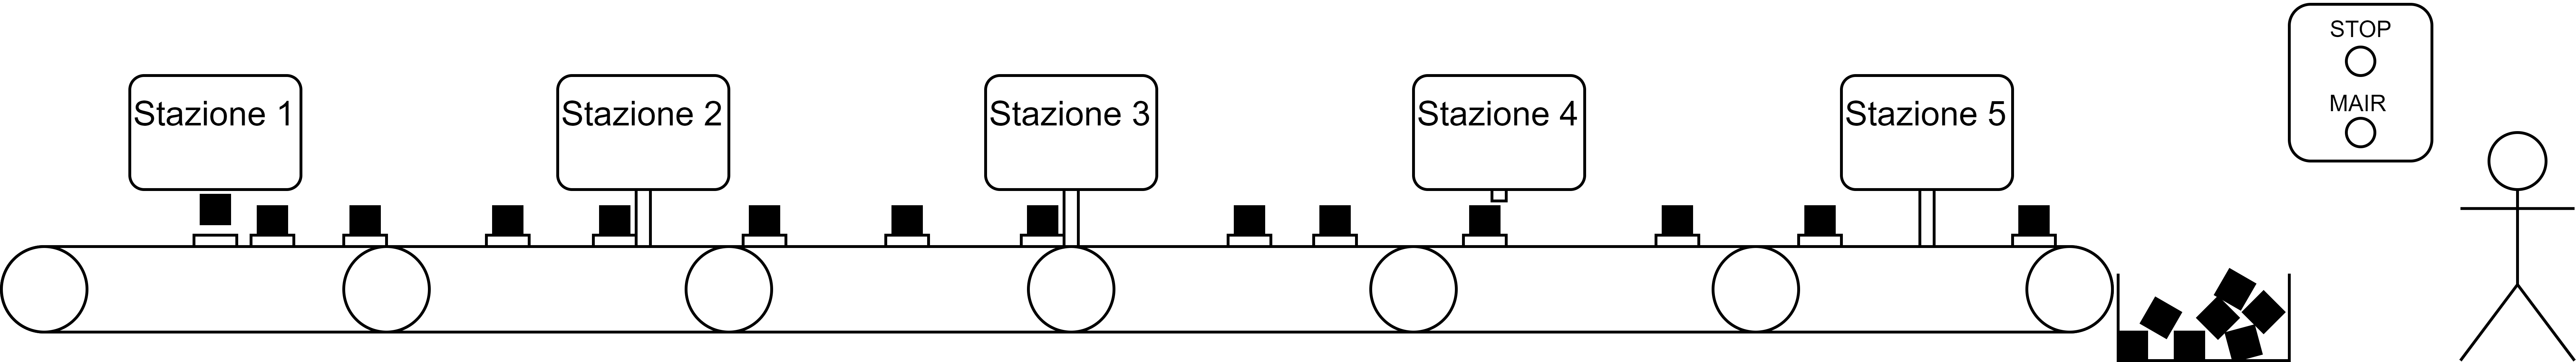
\includegraphics[width = 1 \linewidth]{Diagrammi/TestoStrutturato-schematico.png}
    \caption{Schema di funzionamento}
    \label{fig:schematico}
\end{figure}
\section{Itroduzione}
Il sistema preso in considerazione è una linea di produzione a 5 stazioni [figura \ref{fig:schematico}].
Il pezzo inizialmente viene posizionato sopra un pallet dalla stazione 1; in seguito subisce diverse lavorazioni da parte delle stazioni: 2, 3 e 5 (saldatura, foratura e avvitatura); infine la stazione 5 esegue un controllo di qualità per poi scaricare il pezzo in un contenitore.
\\

Le stazioni saranno di due principali tipologie:
\begin{itemize}
    \item \textbf{Temporizzate}, stazioni: 2, 3 e 4; esse finiranno l'azione allo scadere di un tempo determinato.
    \item \textbf{A evento}, stazioni: 1 e 5; le quali, a seguito di un evento, "presenza pezzo" (stazione 1) oppure "controllo qualità eseguito" (stazione 5), termineranno l'operazione.
\end{itemize}

Inoltre si deve gestire la manutenzione, effettuata ogni 10 pz lavorati.

\section{Assunzioni}
Le assunzioni con cui abbiamo lavorato sono:
\begin{enumerate}
    \item Le fotocellule STAZ\_\# (con \# il numero della stazione) saranno pari a \textit{FALSE} se il pezzo non è presente; mentre rimarranno a \textit{TRUE} per tutta la durata della lavorazione, quindi finché il pezzo non abbandona le stazioni.

    \item L'uscita dalla stazione, da parte di un pezzo, non implica l'accensione della stazione successiva. Questo si traduce nel nostro codice come: quando una stazione si disattiva, la stazione successiva non si accende automaticamente, ma lo si dovrà fare manualmente attivando la fotocellula. Questa scelta è dovuta al fatto che alcune stazioni sono più lente di altre, generando così delle "code"; questo causerebbe difficoltà nella gestione del programma qualora dovesse succedere che una stazione, per esempio STAZ\_3, è ancora in lavorazione mentre la precedente, STAZ\_2, finisce di lavorare, con l'effetto di perdere virtualmente un pezzo.

    Questa assunzione ha comportato l'aggiunta: dell'assunzione numero \ref{ass:3} e dell'utilizzo di un contatore in più (spiegato meglio nella sezione \ref{sec:problematiche}).

    \item I pezzi possono entrare solo dalla prima stazione e uscire dall'ultima, questa assunzione, assieme al secondo contatore, verrà utilizzata per gestire la manutezione.
    \label{ass:3}
\end{enumerate}


\section{Funzione principale}
\begin{figure}
    \centering
    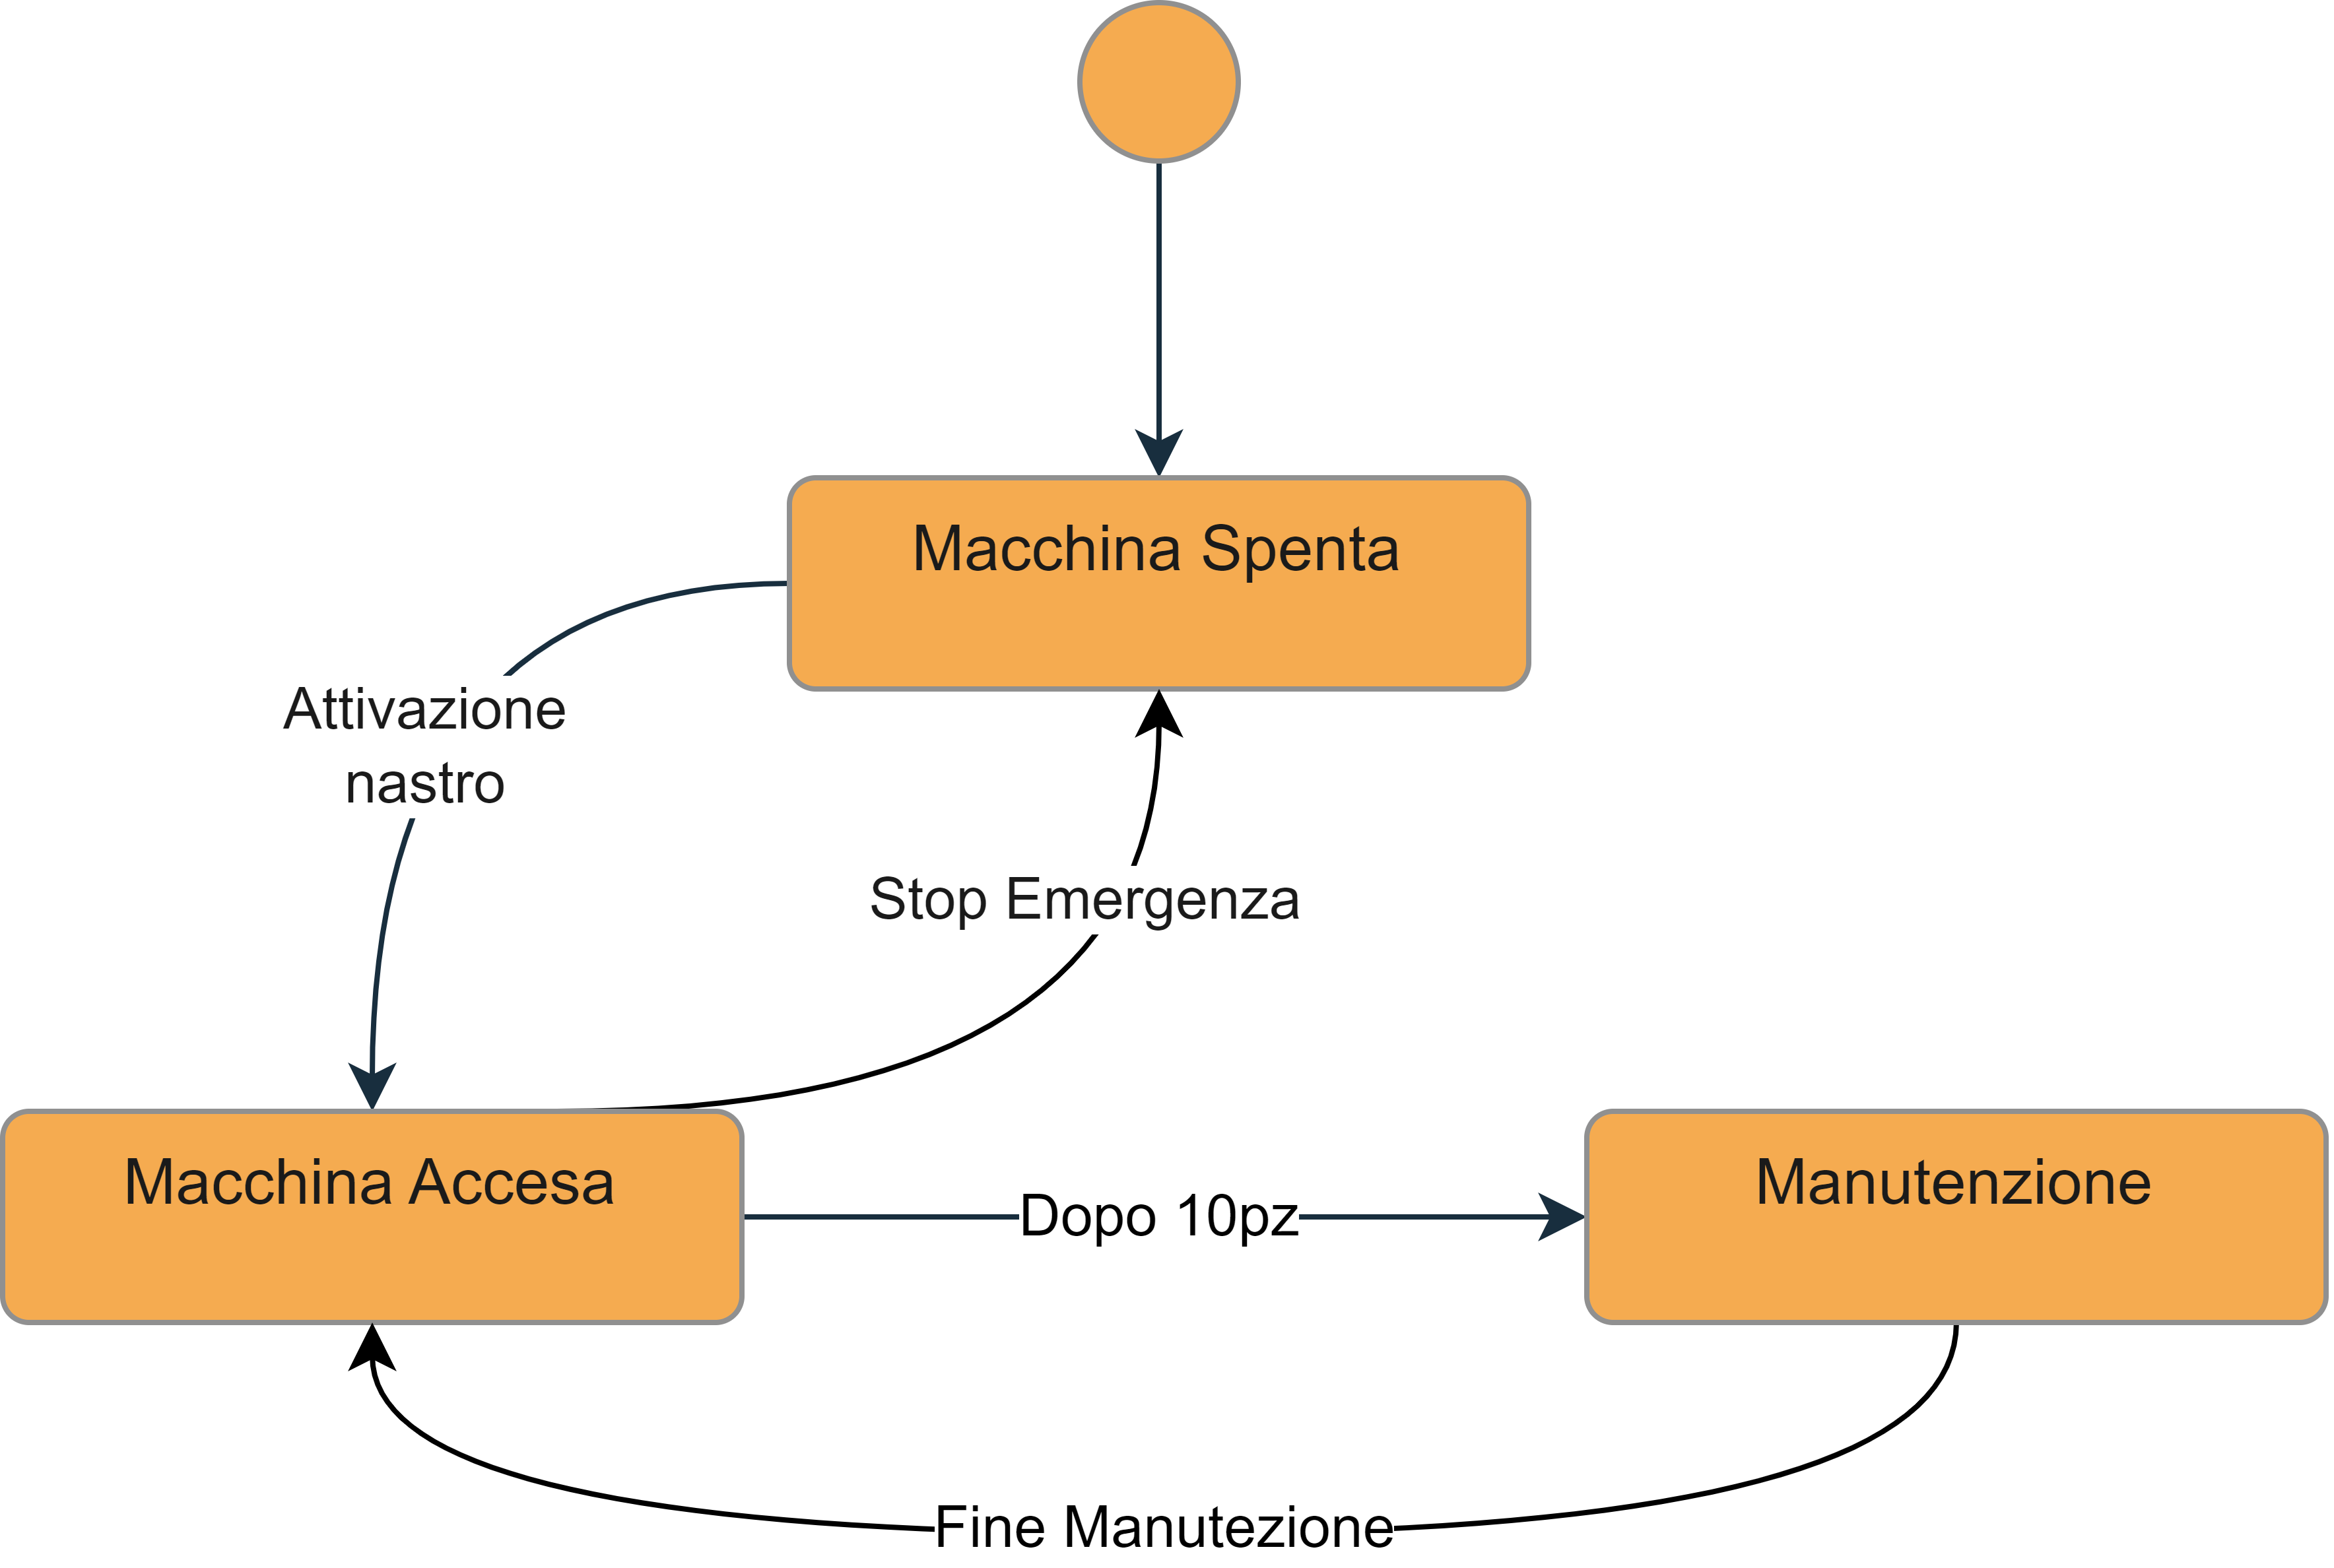
\includegraphics[width = 1 \linewidth]{Diagrammi/TestoStrutturato-main.png}
    \caption{\textit{PROGRAM\_CYCLIC}}
    \label{fig:main}
\end{figure}
La sruttura della funzione principale, \textit{PROGRAM\_CYCLIC}, viene descritta dalla figura \ref{fig:main}. In particolare abbiamo individuato nel sistema tre situazioni diverse:
\begin{itemize}
    \item \textbf{Stato di Fermo}: Tutti gli azionamenti sono spenti, anche se ci sono pezzi sul nastro.
    \item \textbf{Impianto Acceso}: Le stazioni si accendono se è presente un pezzo nella loro zona di lavoro.
    \item \textbf{Stato di Manutenzione}: Tutte le stazioni sono spente perché è richiesta la manutenzione.
\end{itemize}
Il codice lo si può trovare nella sezione \ref{sec:codice_main}.  

\section{Funzione gestione delle stazioni}
\begin{figure}[t]
    \centering
    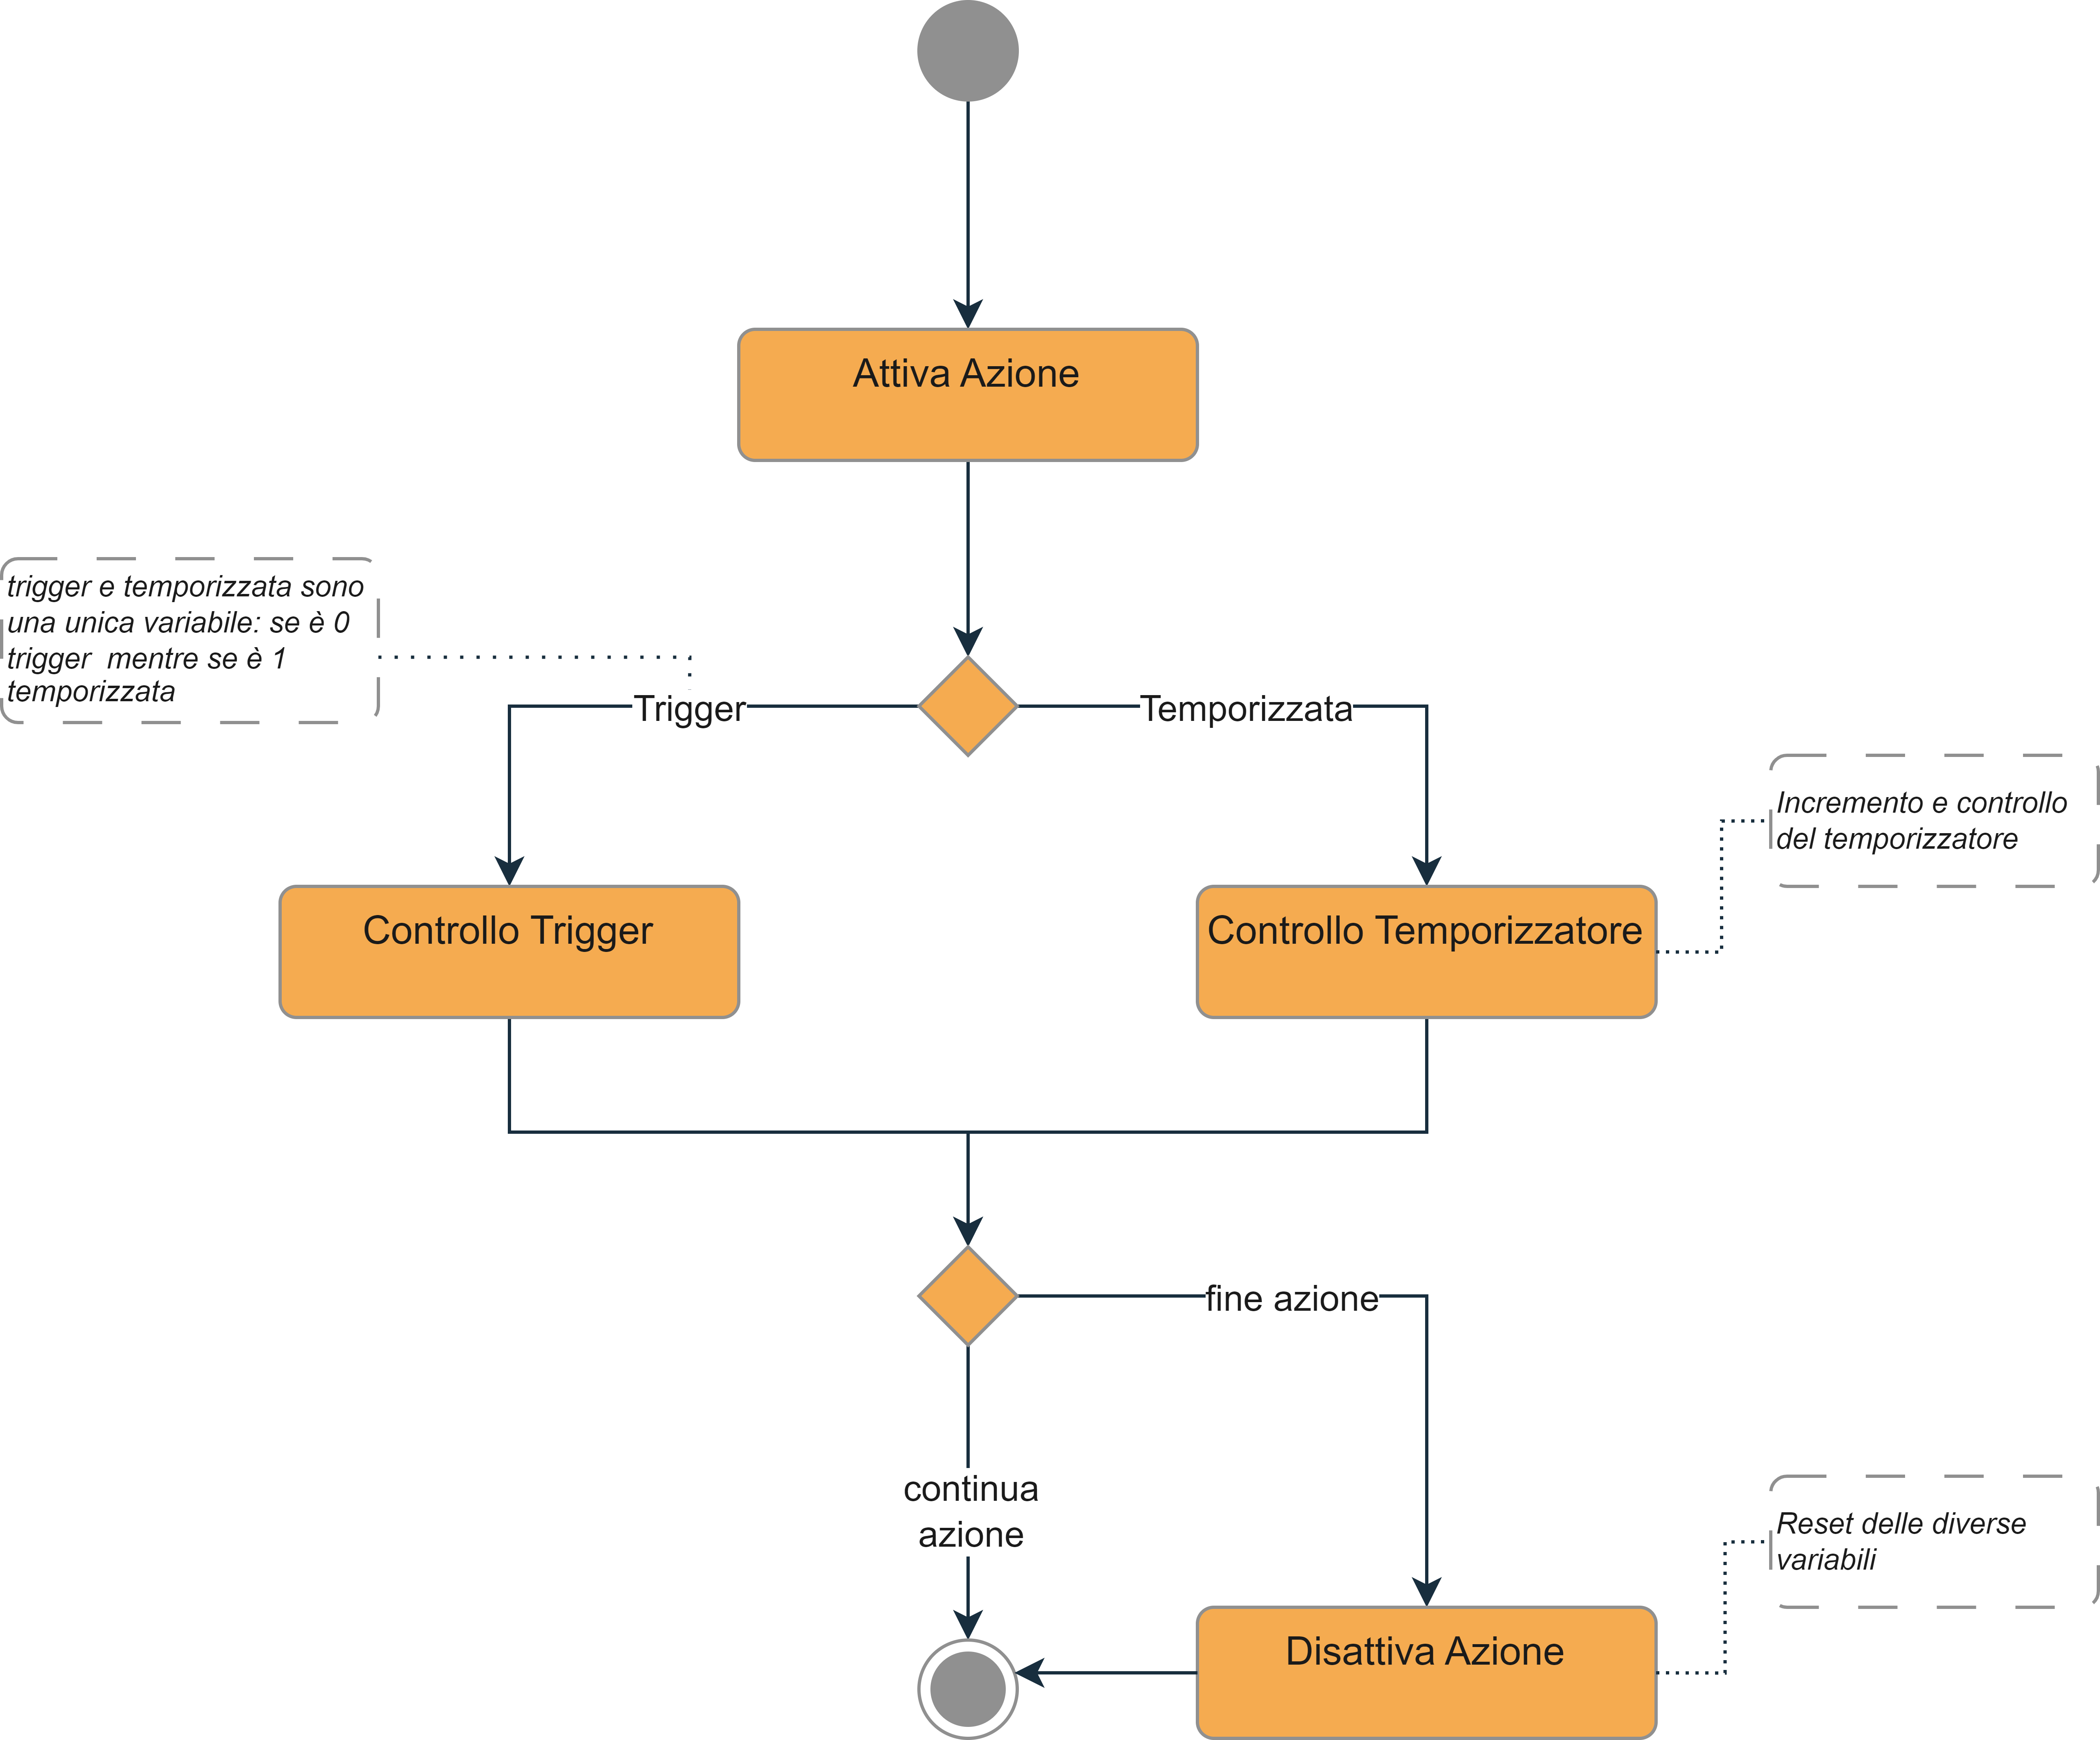
\includegraphics[width = 1 \linewidth]{Diagrammi/TestoStrutturato-funzione.png}
    \caption{Funzione \textit{GESTIONE\_STAZIONE}}
    \label{fig:funzione}
\end{figure}

Per la gestione delle singole stazioni, lo schema di funzionamento è descritto dallo schema \ref{fig:funzione}. Essa all'ingresso attiverà la stazione (se non l'ha già fatto) e, in base alla tipologia di stazione (temporizzata o a evento), eseguirà il controllo: se la stazione si deve spegnere o no.
\\
Gli input e gli output della funzione sono descritti nella tabella \ref{tab:funzione}.
\begin{table}[H]
    \centering
    \begin{tabular}{l l l l }
        \toprule
        \textbf{Nome} & \textbf{Tipologia} & \textbf{Descrizione}                              \\
        \midrule
        \midrule
        TIPO          & Input              & Tipologia di stazione: a evento 0 e               \\
                      &                    & temporizzata 1                                    \\
        \midrule
        TEMPO         & Input              & Il tempo di attivazione, nel caso di stazione     \\
                      &                    & temporizzata                                      \\
        \midrule
        TRIGGER       & Input              & Il trigger che disattiva la stazione, nel caso di \\
                      &                    & stazione a evento                                 \\
        \midrule
        AZIONE        & Input e Output     & L'azione che svolge la stazione                   \\
        \bottomrule
    \end{tabular}
    \caption{Descrizione ingressi e uscite della funzione che gestisce le stazioni}
    \label{tab:funzione}
\end{table}


\section{Problematiche}
\label{sec:problematiche}
La probelmatica principale che abbiamo riscontrato durante lo svolgimento è stata nella gestione della manutenzione. Il problema è dovuto al fatto che le stazioni, per nostra assunzione, non lavorano strettamente in modo sequenziale, o meglio, nella realtà se un pezzo esce da una stazione allora esso sicuramente entrerà nella successiva (il fatto che esca non implica l'ingresso nell'altra, magari ci sono altri pezzi in coda). Quindi, come spiegato in precedenza, l'ingresso si deve fare manualmente (anche perché in questo modo le stazioni lavorano in modo totalmente indipendente tra di esse).
\\

La difficoltà è stata nel contare quanti pezzi sono passati all'ultima stazione, problema che inizialmente abbiamo risolto con un contatore alla fine; ma con l'obbiettivo (posto da noi) di avere la linea scarica quando si va in manutenzione, dovevamo bloccare i pezzi a monte, quindi, il contatore lo abbiamo spostato alla prima stazione. Ciò comportava il problema di capire quando entrare nello stato di manutenzione; supporre che la linea era scarica quando tutte le stazioni erano disattivate non era giusto, magari qualche pezzo stava transitando ancora da una stazione all'altra. Quindi abbiamo risolto inserendo: un sencondo contatore all'uscita dell'ultima stazione e l'assunzione numero: \ref{ass:3}.
\\

Ricapitolando: il primo contatore blocca l'ingresso dell'undicesimo pezzo e il secondo contatore, posto all'ultima stazione il quale segnala che sono passati tutti i pezzi (linea scarica), gestisce il cambio di stato in manutenzione.


\section{Codice}
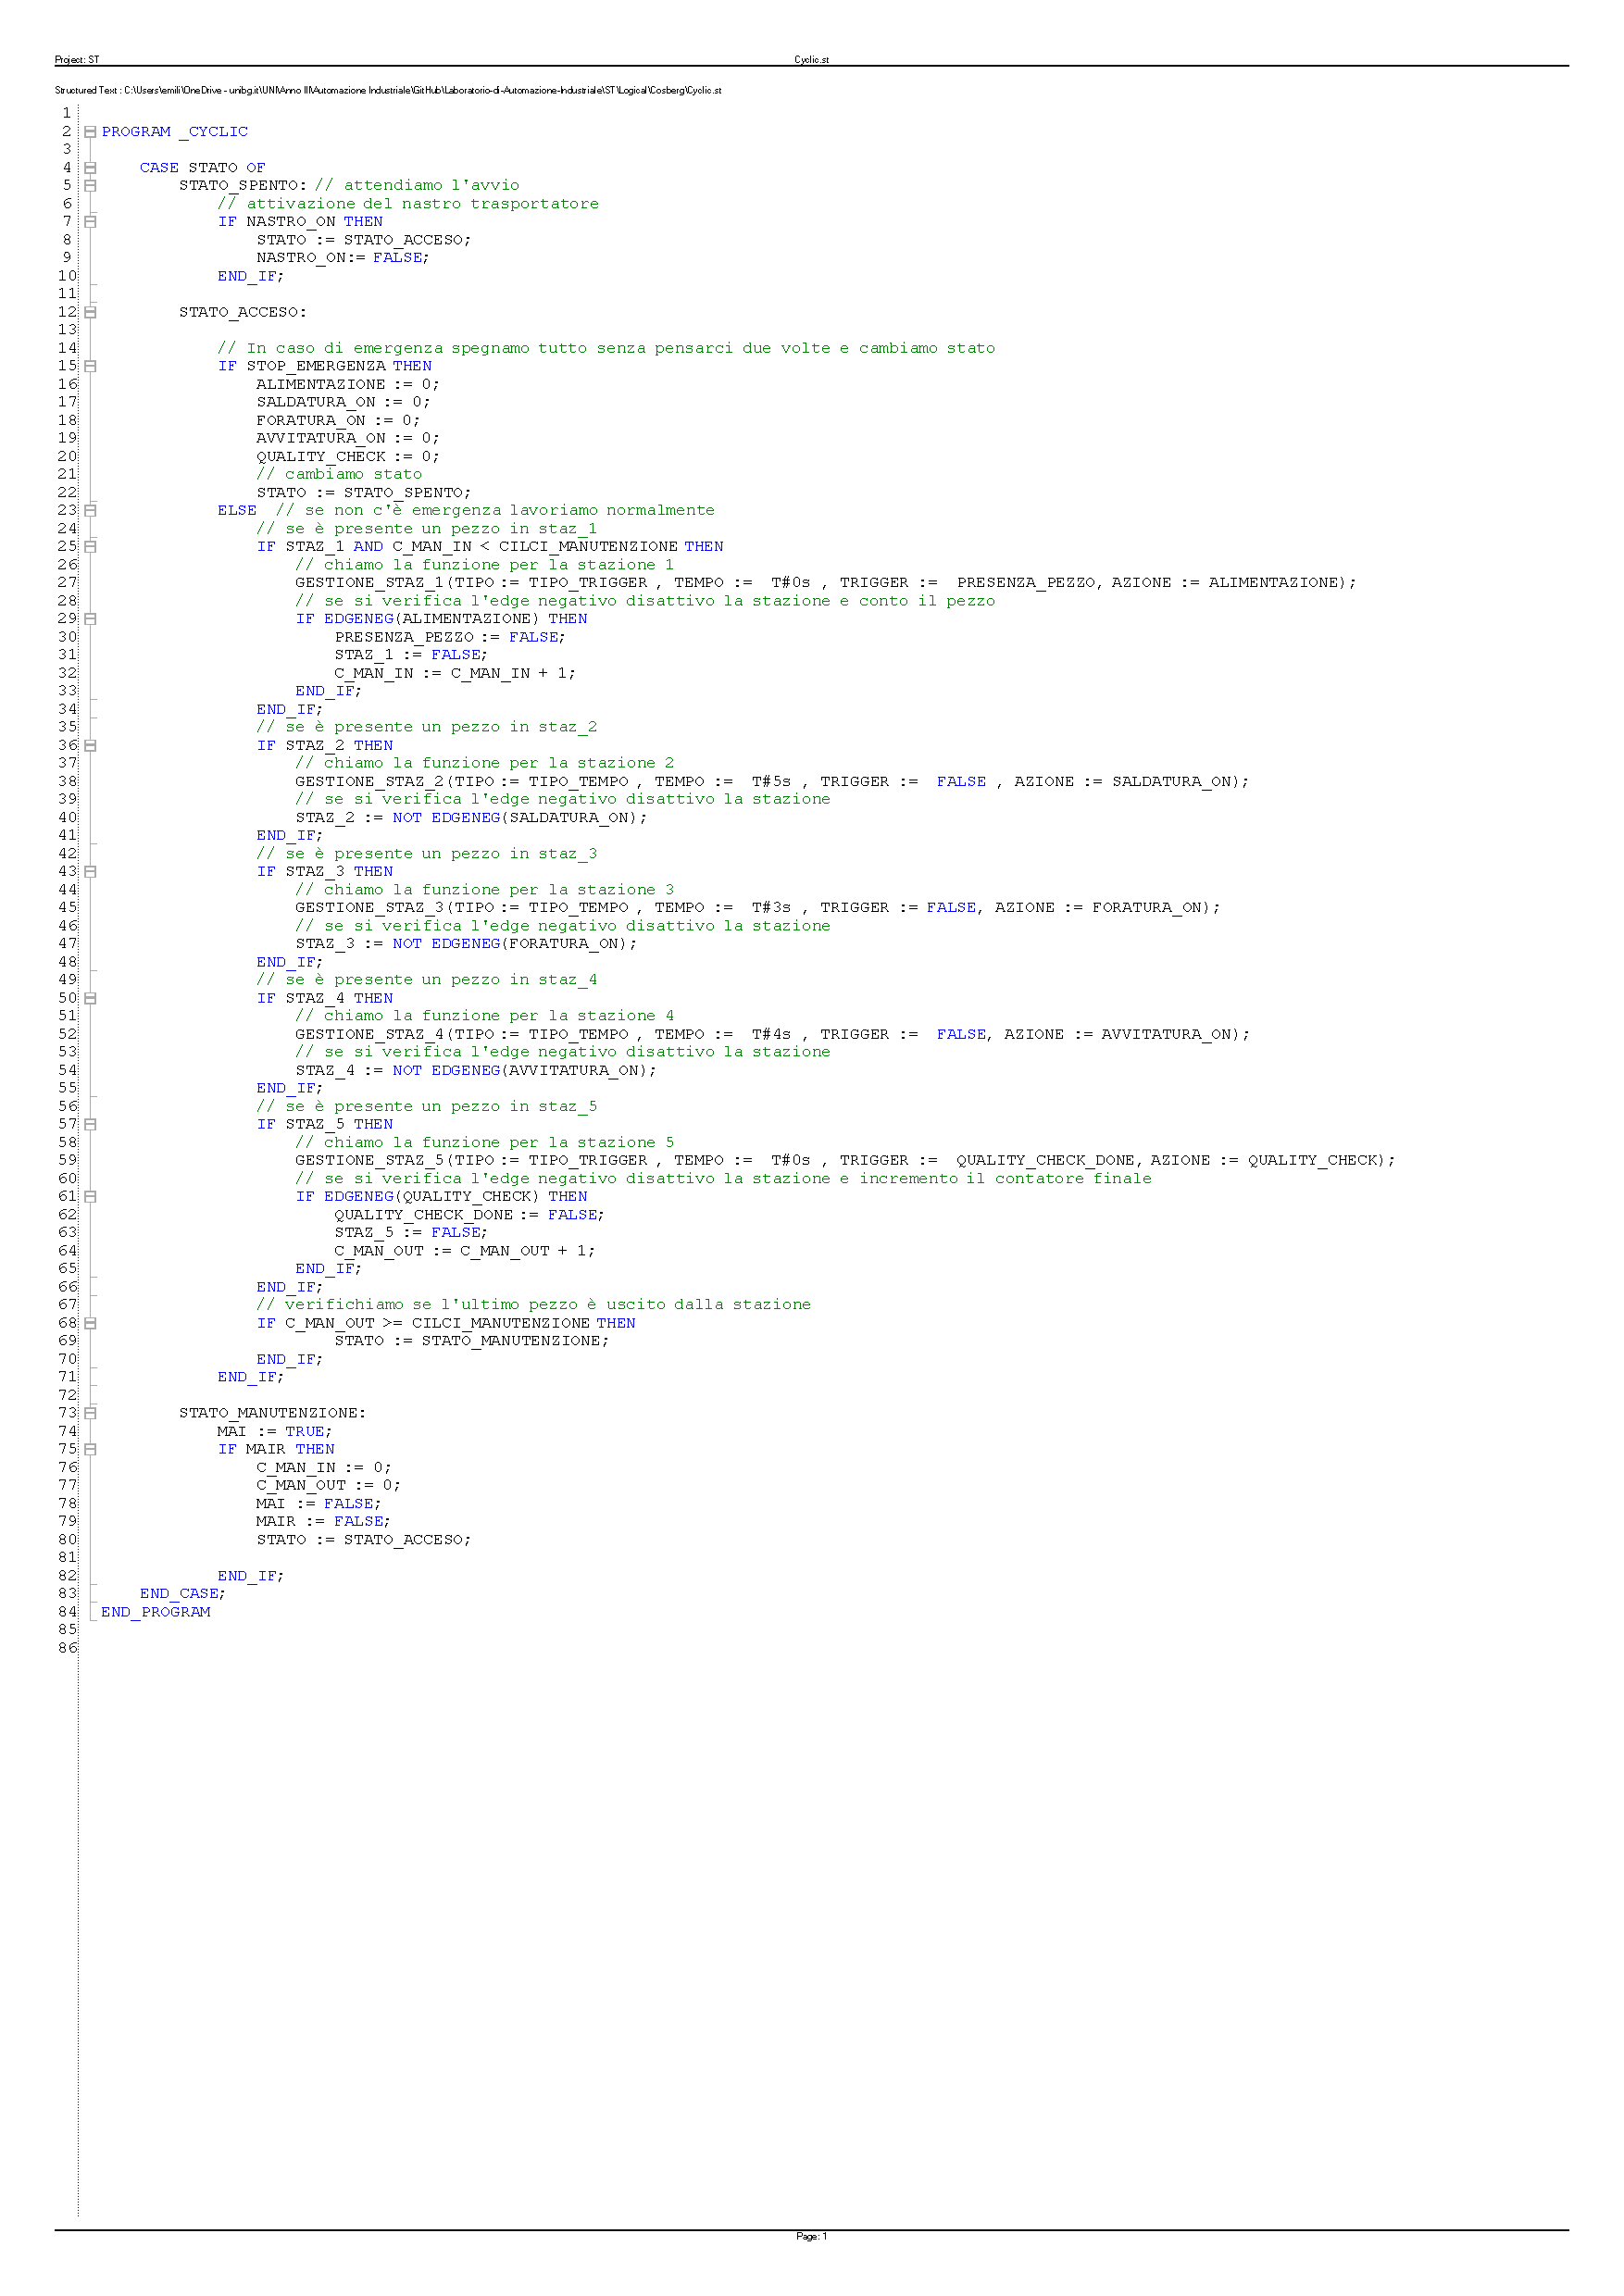
\includepdf[pages=-]{Codice/Main.pdf}
\label{sec:codice_main}

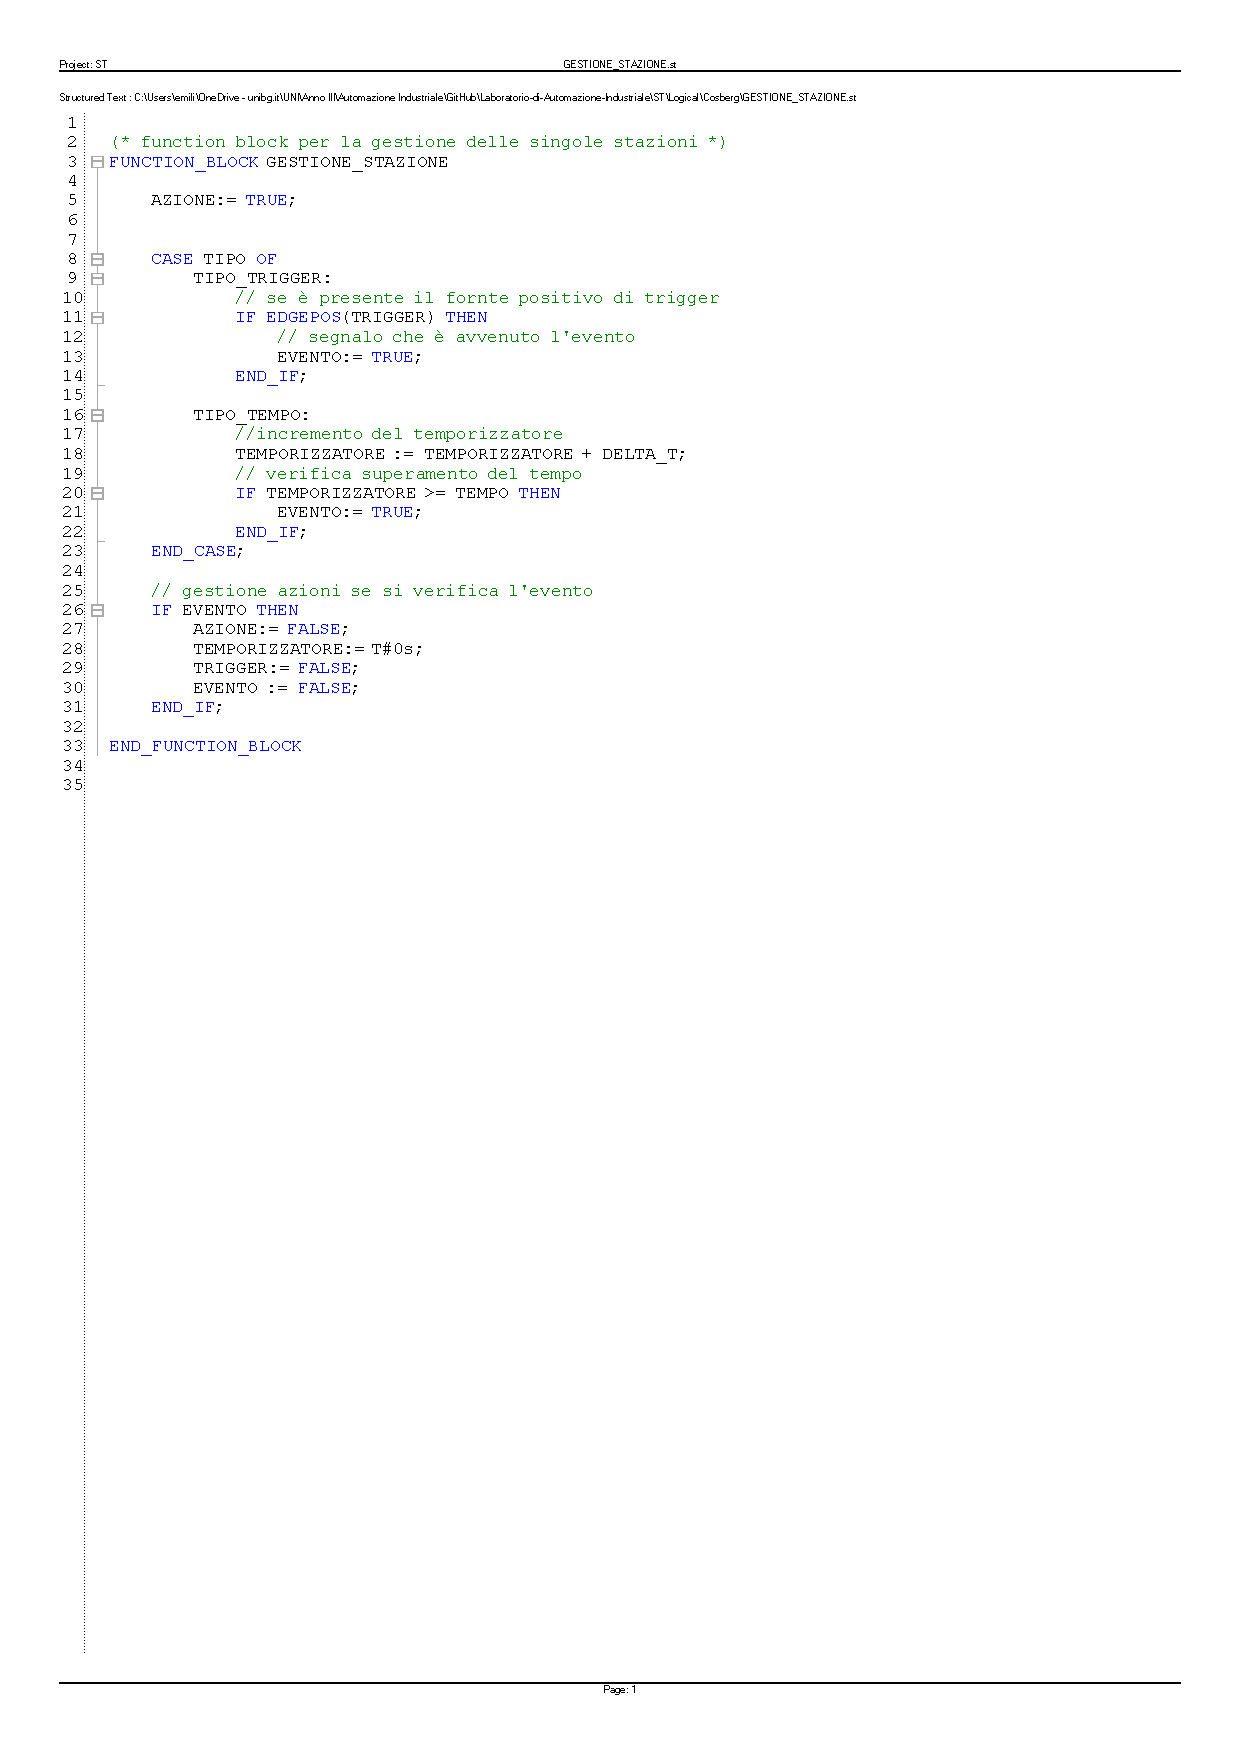
\includepdf[pages=-]{Codice/Funzione.pdf}
\label{sec:codice_funzione}



\end{document}